\documentclass[]{article}
\usepackage{lmodern}
\usepackage{setspace}
\setstretch{2}
\usepackage{amssymb,amsmath}
\usepackage{ifxetex,ifluatex}
\usepackage{fixltx2e} % provides \textsubscript
\ifnum 0\ifxetex 1\fi\ifluatex 1\fi=0 % if pdftex
  \usepackage[T1]{fontenc}
  \usepackage[utf8]{inputenc}
\else % if luatex or xelatex
  \ifxetex
    \usepackage{mathspec}
  \else
    \usepackage{fontspec}
  \fi
  \defaultfontfeatures{Ligatures=TeX,Scale=MatchLowercase}
\fi
% use upquote if available, for straight quotes in verbatim environments
\IfFileExists{upquote.sty}{\usepackage{upquote}}{}
% use microtype if available
\IfFileExists{microtype.sty}{%
\usepackage{microtype}
\UseMicrotypeSet[protrusion]{basicmath} % disable protrusion for tt fonts
}{}
\usepackage[margin = 1in]{geometry}
\usepackage{hyperref}
\hypersetup{unicode=true,
            pdfborder={0 0 0},
            breaklinks=true}
\urlstyle{same}  % don't use monospace font for urls
\usepackage{longtable,booktabs}
\usepackage{graphicx,grffile}
\makeatletter
\def\maxwidth{\ifdim\Gin@nat@width>\linewidth\linewidth\else\Gin@nat@width\fi}
\def\maxheight{\ifdim\Gin@nat@height>\textheight\textheight\else\Gin@nat@height\fi}
\makeatother
% Scale images if necessary, so that they will not overflow the page
% margins by default, and it is still possible to overwrite the defaults
% using explicit options in \includegraphics[width, height, ...]{}
\setkeys{Gin}{width=\maxwidth,height=\maxheight,keepaspectratio}
\IfFileExists{parskip.sty}{%
\usepackage{parskip}
}{% else
\setlength{\parindent}{0pt}
\setlength{\parskip}{6pt plus 2pt minus 1pt}
}
\setlength{\emergencystretch}{3em}  % prevent overfull lines
\providecommand{\tightlist}{%
  \setlength{\itemsep}{0pt}\setlength{\parskip}{0pt}}
\setcounter{secnumdepth}{5}
% Redefines (sub)paragraphs to behave more like sections
\ifx\paragraph\undefined\else
\let\oldparagraph\paragraph
\renewcommand{\paragraph}[1]{\oldparagraph{#1}\mbox{}}
\fi
\ifx\subparagraph\undefined\else
\let\oldsubparagraph\subparagraph
\renewcommand{\subparagraph}[1]{\oldsubparagraph{#1}\mbox{}}
\fi

%%% Use protect on footnotes to avoid problems with footnotes in titles
\let\rmarkdownfootnote\footnote%
\def\footnote{\protect\rmarkdownfootnote}

%%% Change title format to be more compact
\usepackage{titling}

% Create subtitle command for use in maketitle
\providecommand{\subtitle}[1]{
  \posttitle{
    \begin{center}\large#1\end{center}
    }
}

\setlength{\droptitle}{-2em}

  \title{}
    \pretitle{\vspace{\droptitle}}
  \posttitle{}
    \author{}
    \preauthor{}\postauthor{}
    \date{}
    \predate{}\postdate{}
  
\usepackage[left]{lineno}
\linenumbers

\begin{document}

Running head: DATELIFE: REVEALING THE DATED TREE OF LIFE

Title: DateLife: Leveraging databases and analytical tools to reveal the dated Tree of Life

Authors: Luna L. Sánchez-Reyes\textsuperscript{1}, Brian C. O'Meara\textsuperscript{1}

Correspondence address:

\begin{enumerate}
\def\labelenumi{\arabic{enumi}.}
\tightlist
\item
  \emph{Department of Ecology and Evolutionary Biology, University of Tennessee, Knoxville, 425 Hesler Biology Building, Knoxville, TN 37996, USA}
\end{enumerate}

Corresponding authors: \href{mailto:sanchez.reyes.luna@gmail.com}{\nolinkurl{sanchez.reyes.luna@gmail.com}}, \href{mailto:bomeara@utk.edu}{\nolinkurl{bomeara@utk.edu}}

\newpage

\textbf{abstract.-}
The combination of new analytical techniques, availability of more fossil and molecular
data, and better practices in data sharing has resulted in a steady accumulation
of chronograms in public and open databases such as TreeBASE, Dryad, and Open Tree
of Life, for a large quantity and diversity of organisms in the last decades. However, time of lineage divergence data remains difficult to be obtained and synthesized for many biologists and the non-academic community, despite its importance in many areas of research, education and science communication. \texttt{datelife} is a service implemented via an R package and a web site
(\url{http://www.datelife.org/}) for efficient reuse, summary and reanalysis of expert, published data on time of lineage divergence. The main workflow starts with at least two taxon names as input, either as tip labels on a tree, or as a simple comma separated character string. A name search is then performed across the chronogram database and positively identified source trees are pruned to maintain queried taxa only and stored as a named list of patristic distance matrices. Source chronogram data can be summarised using branch length summary statitiscs or variance minimising approaches to generate a single summary chronogram. Source chronogram data can also be used as calibration points to date a tree containing some or all names from the initial query. If there is no information available for any queried taxa, data can be simulated. All source and summary chronograms can be saved in formats that permit easy reuse and reanalysis. Summary and newly generated trees are potentially useful to evaluate evolutionary hypothesis in different areas of research in biology. How well this trees work for this purpose still needs to be tested. \texttt{datelife} will be useful to increase awereness on the existing variation in expert time of divergence data, and might foster exploration of the effect of alternative divergence time hypothesis on the results of analyses, nurturing a culture of more cautious interpretation of evolutionary results.

\textbf{Keywords:} Tree; Phylogeny; Scaling; Dating; Ages; Divergence times; Open Science; Congruification; Supertree; Calibrations

\newpage

Time of lineage divergence constitutes a fundamental piece of information for evolutionary
understanding in many areas of research, from developmental to conservation biology (Felsenstein \protect\hyperlink{ref-Felsenstein1985a}{1985}; Webb \protect\hyperlink{ref-Webb2000}{2000}), from historical biogeography to species diversification studies (Posadas et al. \protect\hyperlink{ref-posadas2006historical}{2006}; Morlon \protect\hyperlink{ref-Morlon2014}{2014}). The primary information needed for time of lineage divergence estimation comes from the fossil record. Coupled to molecular phylogenies (and more recently to morphological data), the time of divergence of extant and extinct lineages is reconstructed with molecular dating methods.
Probably encouraged by the great developments in DNA sequencing techniques, phylogenetic inference and molecular dating methods, the number of studies publishing phylogenies with branch lengths proportional to geologic time (hereafter chronograms) have constantly increased in number for the last two decades (Kumar et al. \protect\hyperlink{ref-Kumar2017}{2017}).
Still, generating a chronogram is not an easy task unless you have specialized training. That's why there has been an urge for promoting and facilitating reuse of the vast amount of phylogenetic and time of lineage divergence data that has been generated and made available in publications, for the advantage of research relying on this information (Webb and Donoghue \protect\hyperlink{ref-webb2005phylomatic}{2005}; Stoltzfus et al. \protect\hyperlink{ref-Stoltzfus2013}{2013}).

Wide interest from the scientific community to make information from phylogenies in general and chronograms in particular available for consultation and reuse has spurred the creation of public platforms with various goals and characteristics. TreeBASE (Morell \protect\hyperlink{ref-morell1996roots}{1996}; Piel et al. \protect\hyperlink{ref-Piel2002}{2002}), the Dryad repository (\url{http://datadryad.org/}), and the Open Tree of Life (OToL; Hinchliff et al. \protect\hyperlink{ref-Hinchliff2015}{2015}) platforms store and make available published phylogenies and chronograms for easy scientific reuse. All of them can be queried using automatised web procedures, which permit personalised, large scale queries that are also very fast.
OToL stores trees with branch length information from a wide range of living organisms, implementing a metadata structure that stores the branch length units (i.e., time or relative susbtitution rates). Treebase and Dryad repositories also contain trees from all groups of life, but the former does not store branch length information and Dryad stores many other types of biological data using metadata that does not allow automatic distinction of types of trees and branch length units, impairing the automatised access to time of lineage divergence information.

Besides keeping a repository to easily store and share expert phylogenetic and chronogram knowledge, OToL also has the primary goal of synthesising all trees in their repository to expose to the community a single tree of all life depicting the phylogenetic relationships among known lineages.
All or parts of this synthetic tree can be reused for any purpose. However, it currently only focus on synthesizing tree topology, meaning that it does not expose branch length data of any type.
The Timetree of Life project focuses on the synthesis of a single chronogram of life (Hedges et al. \protect\hyperlink{ref-Hedges2006}{2006}). However, the thousands of chronograms they have compiled for synthesis are only publicly available for visual examination in their website or for download as images, but not for scientific reuse or reanalysis. The latest version of their synthetic chronogram (Kumar et al. \protect\hyperlink{ref-Kumar2017}{2017}) can be queried only through their website in a non-automatised fashion, and only subsets of it can be reused for analyses with the permission of the authors.
Other platforms such as SuperSmart (Antonelli et al. \protect\hyperlink{ref-antonelli2017supersmart}{2017}) and phylogenerator (Pearse and Purvis \protect\hyperlink{ref-pearse2013phylogenerator}{2013}) are focused in automatised \emph{de novo} chronogram inference, by reusing DNA sequence data to reconstruct phylogenetic trees. However, expert fossil information necessary for subsequent molecular dating analyses still needs to be compiled and curated by the user, rendering them a challenging tool to obtain data on time of lineage divergence for the non-specialist. Moreover, these tools do not provide information from already existent expert chronograms.

A tool for efficient reuse of expert, published data on time of lineage divergence should have an open and fuly public chronogram database storing data in a format suitable for scientific reuse, an automatised way of accessing the information, and straightforward means of comparing and summarizing chronogram information as needed by the user.
A prototype service aiming to meet this characteristics was developed over a series of hackathons at the National Evolutionary Synthesis Center (Stoltzfus et al. \protect\hyperlink{ref-Stoltzfus2013}{2013}).
In here we present the formal description and implementation of the \texttt{datelife} service, constituted by an R package and a web site (\url{http://www.datelife.org/}). There is still much room for improvement, and flaws and limitations are addressed below. We strived for the current implementation of \texttt{datelife} to perform the basic tasks described above, featuring a system for maintenance of an open database of chronograms pulled from public repositories, methods to summarize and compare source chronograms, and new functions to visualize and graphically compare source and summary chronograms.
R packages for benchmarking of functionalities and demonstrating services were also developed and made available.

\begin{center}
\textsc{Description}
\end{center}

The basic \texttt{datelife} workflow is shown in figure \ref{fig:workflow} and consists of:

\begin{enumerate}
\item A user providing at least two taxon names as input, either as tip labels on a tree, or as a simple comma separated character string. The tree can be in newick or phylo format, and can be with or without branch lengths.
\item A name search is then performed across the chronogram database; source trees with at least two matching input names are identified; all other taxa that do not match the original query are then dropped from the positively identified source trees --these pruned chronograms are hereafter referred as source chronograms; finally, each source chronogram is transformed to a patristic matrix named by the citation of the original study. This format facilitates and greatly speeds up all further analyses and summarising algorithms.
\item  The user can obtain different summary information from the source chronograms including: a) all source chronogram ages, b) maximum ages of source chronograms, c) citations of studies where source chronograms were originally published, d) a summary table with all of the above, e) a single summary tree of all or a subset of source chronograms, and f) a report of succesful matches of input taxon names across source chronograms. Summary information can be used to make decisions on the next steps of the workflow. 
\item  Source chronogram data can be used as calibration points to date a tree with or without branch lengths containing some or all names from the initial query. %<!--, a taxonomic tree-->
\item  If there is no information available for any queried taxa, users can also simulate both age and phylogenetic data for this missing taxa with a variety of algorithms described below.
\item  Finally, users can easily save all source and summary chronograms in formats that permit easy reuse and reanalyses (newick and R `phylo` format), as well as view and compare results graphically, or construct their own graphs using inbuilt `datelife` graphic generation functions.
\end{enumerate}

To gather, process, and present information, \texttt{datelife} builds up from functions
available in several R packages including rotl (Michonneau et al. \protect\hyperlink{ref-Michonneau2016}{2016}), ape (Paradis et al. \protect\hyperlink{ref-Paradis2004}{2004}),
geiger (Harmon et al. \protect\hyperlink{ref-Harmon2008}{2008}), paleotree (Bapst \protect\hyperlink{ref-Bapst2012a}{2012}), bold (Chamberlain \protect\hyperlink{ref-Chamberlain2018}{2018}), phytools (Revell \protect\hyperlink{ref-Revell2012}{2012}), taxize (Chamberlain and Szöcs \protect\hyperlink{ref-Chamberlain2013}{2013}; Chamberlain \protect\hyperlink{ref-Chamberlain2018}{2018}), phyloch (Heibl \protect\hyperlink{ref-Heibl2008}{2008}), phylocomr (Ooms and Chamberlain \protect\hyperlink{ref-Ooms2018}{2018}) and rphylotastic (O'Meara et al. \protect\hyperlink{ref-Omeara2019}{2019}).

A \texttt{datelife} search currently accepts scientific names only. It can be any named clade or binomial specific.
Chronogram search is performed at the species level, so when input names correspond
to named clades, \texttt{datelife} pulls all accepted species names within the
clade from OToL's reference taxonomy to perform the search.
Searches at the infraspecies level are not currently allowed, so input names belonging to subspecies or any other infraspecific category are collapsed to the species level.
\texttt{datelife} processes input names with the taxon name resolution service (TNRS; Boyle et al. \protect\hyperlink{ref-Boyle2013}{2013}),
which corrects potentially misspelled names and typos, and standardizes spelling
variations and synonyms , increasing the probability to correctly find the
queried taxa in \texttt{datelife}'s chronogram database.

The chronogram search is performed across \texttt{datelife}'s chronogram database which is assembled from OToL's tree repository. Compared to other existing open tree repositories OToL's metadata rich tree store is the only one that supports search, identification, and handling of chronograms in an automatised fashion. Also, all their chronograms come from peer-reviewed published studies generated by specialists in the targeted lineages, arguably representing expert knowledge on time of lineage divergence.

Information from source chronograms can be summarised with a summary statistic of tree branch
lengths (such as median or mean) or using the Super Distance Matrix (SDM) approach for supertree reconstruction (Criscuolo et al. \protect\hyperlink{ref-Criscuolo2006}{2006}).
The resulting summary patristic distance matrix could be clustered with classic algorithms. However, we noticed that the resulting trees are often non-ultrameric and do not reflect the source chronogram data (see datelife\_examples package). Instead, we obtained a distribution of age data from the summary matrix available for nodes on a consensus tree. The Branch Length Adjuster (BLADJ) algorithm (Webb et al. \protect\hyperlink{ref-Webb2008}{2008}) was then used to distribute node ages evenly over the consensus tree, minimizing age variance in the resulting chronogram.

For tree dating, the congruification algorithm described by Eastman et al. (\protect\hyperlink{ref-Eastman2013}{2013})
is implemented to find shared nodes between trees (congruent nodes). The ages of these nodes are then used as calibrations to date any given tree. Currently implemented methods for tree dating are BLADJ, MrBayes (Huelsenbeck and Ronquist \protect\hyperlink{ref-Huelsenbeck2001}{2001}; Ronquist and Huelsenbeck \protect\hyperlink{ref-Ronquist2003}{2003}) and PATHd8 (Britton et al. \protect\hyperlink{ref-Britton2007}{2007}), a non-clock, rate-smoothing dating method.

\begin{center}
\textsc{Benchmark}
\end{center}

\texttt{datelife}'s code speed was tested on an Apple iMac
with one 3.4 GHz Intel Core i5 processor.
We registered variation in computing time of query processing and search through the database relative to number of queried taxon names.
Query processing increases roughly linearly with number of input taxon names, and
increases considerably if TNRS service is activated. Up to ten thousand names can be processed and searched in less than 30 minutes. A name search through the chronogram database with an already processed query can be performed in less than a minute, even with a very large number of taxon names (Fig. \ref{fig:runtime1}).
\texttt{datelife}'s code performance was evaluated with a set of unit tests designed and
implemented with the R package testthat (R Core Team \protect\hyperlink{ref-RCoreTeam2018}{2018}) that were run locally
--using the devtools package (R Core Team \protect\hyperlink{ref-RCoreTeam2018}{2018}), and on a public server --via
GitHub, using the continuous integration tool Travis CI (\url{https://travis-ci.org}). At
present, unit tests cover more than 50\% of \texttt{datelife}'s code (\url{https://codecov.io/gh/phylotastic/datelife}).

\begin{center}
\textsc{Example}
\end{center}

In this section we demonstrate the types of outputs that can be obtained with \texttt{datelife}, using as an example the bird family Fringillidae of true finches. We performed a higher-taxon search to obtain all data on lineage divergence available in \texttt{datelife}'s database for all recognised species within the Fringillidae (475 spp. according to the Open Tree of Life taxonomy). There are 13 chronograms containing at least two Fringillidae species, published in 9 different studies (Fig. \ref{fig:schronograms1}).
Data from these source chronograms was used to generate two types of summary chronograms, median and SDM. As explained in the \texttt{Description}, data from source chronograms was first summarised into a single distance matrix (using either the median or the SDM method) and then the available node ages were used as calibrations points over a consensus tree topology, to obtain a dated tree with the program BLADJ (Fig. \ref{fig:summaries}). Median summary chronograms are older and have wider variation in maximum ages than chronograms obtained with SDM. In both cases, ages are coherent with source ages.
It is not certain if these chronograms should be used to perform all types of downstream evolutionary analyses and more research is needed in that direction.

Data from source chronograms was also used to date tree topologies with no branch length information and trees with branch lengths in relative substitution rates (Figs. \ref{fig:cvbladj} and \ref{fig:cvbold}). As a form of cross validation, we used tree topologies from each study and calibrated them using information from all other source chronograms. In the absence of branch length data, the ages of internal nodes were approximately recovered in almost all cases (except for studies 3, and 5; Fig. \ref{fig:cvbladj}). Maximum tree ages were only approximately recovered in one case (study 2; Fig. \ref{fig:cvbladj}).
Branch lengths were successfully generated using the BOLD database for all source chronograms. However, dating with PATHd8 (using congruified calibrations) was only successful in
three cases (studies 3, 5, and 9; Fig. \ref{fig:cvbold}). From these, two trees have a different sampling than the original source chronogram, mainly because DNA data for some species is absent from the BOLD. Maximum ages are quite different from source chronograms, but this might be explained also by the differences in sampling between source chronograms and BOLD trees.
More examples and details can be consulted in \url{https://github.com/LunaSare/datelife_examples}.

\begin{center}
\textsc{Flaws, Limitations and Prospects}
\end{center}

The main goal of \texttt{datelife} is to make expert information on time of lineage divergence easily accesible for comparison, reuse, and reanalysis, to researchers in all areas of science and with all levels of expertise in the matter. It is a very fast tool that fulfills the quality of openness and does not require any expert biological knowledge from users --besides the names of the organisms they want to work with-- for any of its functionalities. However, it has many flaws. Some of them can be overcome, some of them might represent limitations.

At the moment, \texttt{datelife}'s chronogram database is not very large, storing 231 chronograms up to the time the manuscript was written. This represents 5.79\% of the largest existing chronogram database, which is unfortunately not open for scientific reuse nor automatised data mining (Kumar et al. \protect\hyperlink{ref-Kumar2017}{2017}). OToL is the only public tree repository from where \texttt{datelife} can currently pull chronograms to construct its database. Other open repositories are not suitable for time of divergence data mining because they either do not store that data (i.e., TreeBASE), or their metadata does not have enough information to allow automatised chronogram searches (i.e., Dryad).
A previous version of TimeTree's synthetic chronogram (Hedges et al. \protect\hyperlink{ref-Hedges2015}{2015}) was made available in OToL repository, hence the amount of lineages represented in datelife's database is at least as substantial as TimeTree's.
This ensures that some information will be available for any given query, but it does not ensure that the full state of knowledge of time of divergence data will be available for any given lineage.
Thus, incorporation of published chronograms available in the Dryad data repository and in supplementary material of journals to \texttt{datelife}'s database is crucial to improve its services.
Methods to automatically mine chronogram data from the Dryad repository could be designed and implemented. However, the unit of branch lengths would still need to be determined by ``hand''.
Consequently, we would like to emphasize on the importance of sharing chronogram data for the scientific community, in repositories that require expert input and manual curation, such as OToL's tree repository.

Another potential concern comes from summary chronograms. We currently summarize all source chronogram data by default. Users can subset source data if they have reasons to favor some or one source chronogram over others. Strictly speaking, a good chronogram should reflect the real time of lineage divergence accurately and precisely. To our knowledge, there is no objective way to determine if an expert chronogram is better than other. Some criteria that have been put forward are the level of lineage sampling and the number of calibrations used. Scientists usually also favor chronograms coming from studies with primary calibrations to ones from secondary calibrations. It has been observed with simulations that divergence times inferred with secondary calibrations are significantly younger than those inferred with primary calibrations in analyses performed with bayesian inference methods when priors are implemented in similar ways in both analyses (Schenk \protect\hyperlink{ref-schenk2016sec}{2016}). Yet, there are different ways to use secondary calibrations and the bias might not be encountered with other dating methods that do not require prior assumptions (such as ML methods). But this remains to be tested.

Furthermore, even chronograms obtained with primary data can be very different, as observed from the comparison of source chronograms in the Fringillidae example.
A large discrepancy in time of lineage divergence across expert knowledge is well known for different groups of organisms (e.g., angiosperms; Magallón et al. \protect\hyperlink{ref-magallon2015metacalibrated}{2015}). Comparison of available chronogram data for a wide range of organisms shown here suggest that this is a widespread phenomenon that requires further attention.
Characteristics of the data used for dating analyses as well as from the output chronogram itself, such as quality of alignement (missing data, GC content), lineage sampling strategy and proportion, phylogenetic and dating inference method, number of fossils used as calibrations, support for nodes and ages, and confidence intervals could be used to score quality of source chronograms. To facilitate subsetting of source chronograms following different criteria, this information should be included as metadata manually entered by curators (as is done in OToL) in the future.
Still, even if all source chronograms have been generated by excellent standards and using similar methods, the evolutionary history they depict might be very different. Hence, summarizing chronograms might imply summarizing evolutionary hypothesis. This could be good from certain point of view, since it could help to get a single global evolutionary history for a lineage. But it could also be bad, since we could be loosing part of the evolutionary history that is only being reflected in some chronograms and not from the summary chronogram.
Ideally, we should still rely on time of lineage divergence data obtained from a single analysis using fossil data as primary sources of calibrations, and using fossils that have already been curated as calibrations to date other trees, which should reflect a more homogeneous evolutionary history (Antonelli et al. \protect\hyperlink{ref-antonelli2017supersmart}{2017}). This will be implemented in future \texttt{datelife} versions.

Synthetic or summary chronograms are being used more and more frequently to study evolutionary hypothesis. We introduce different ways of summarizing time of lineage divergence data, but, are any of these summary chronograms reliable to study evolutionary patterns? The short answer is that we do not know to what extent the summary trees should be used for reanalyses and if there bare areas of research where they can be used more reliably than others. There is evidence that different chronograms will result in very different macroevolutionary histories inferred from them (Title and Rabosky \protect\hyperlink{ref-title2016macrophylogenies}{2016}). In other areas of biological research, such as ecology and conservation biology, it has been indicated that at least some data on lineage divergence represents an improvement for testing alternative hypothesis using phylogenetic distance. It is uncertain, however, how using very different age data could affect the outcomes of these tests, and further research is necessary in this direction.

\begin{center}
\textsc{Conclusions}
\end{center}

Time of lineage divergence information is key to many areas of evolutionary studies: trait evolution,
diversification, biogeography, macroecology and more. Generating this information is difficult,
especially for those who want to use phylogenies but who are not systematists, or
do not have the time to acquire and develop the necessary knowledge and data curation skills
to produce chronograms \emph{de novo}. Knowledge on taxon ages is also crucial for
science communication and education.

\texttt{datelife} allows an easy and fast obtention, as well as comparison of publicly available information
on time of lineage divergence, providing a straightforward way to get an informed idea on the state of knowledge of the time frame of evolution of different regions of the tree of life, allowing identification of regions that require more research or that have conflicting information.
Both summary and newly generated trees are potentially useful to evaluate evolutionary hypothesis in different areas of research. How well this trees work for this purpose still needs to be further tested. If all, \texttt{datelife} helps with awereness on the existing variation in expert time of divergence data, and might foster exploration of the effect of alternative divergence time hypothesis on the results of analyses, nurturing a culture of more cautious interpretation of evolutionary results.

\begin{center}
\textsc{Availability}
\end{center}

\texttt{datelife} is free and open source and it can be used through its current website
\url{http://www.datelife.org/query/}, through its R package, and through Phylotastic's project web portal \url{http://phylo.cs.nmsu.edu:3000/}.
\texttt{datelife}'s website is maintained using RStudio's shiny server and the shiny package open infrastructure, as well as Docker.
\texttt{datelife}'s R package stable version is available
for installation from the CRAN repository (\url{https://cran.r-project.org/package=datelife})
using the command \texttt{install.packages(pkgs\ =\ "datelife")} from within R. Development versions
are available from the GitHub repository (\url{https://github.com/phylotastic/datelife})
and can be installed using the command \texttt{devtools::install\_github("phylotastic/datelife")}.

\begin{center}
\textsc{Supplementary Material}
\end{center}

Code used to generate all versions of this manuscript, the biological examples, as well as the benchmark of functionalities can be found in GitHub repositories at \url{https://github.com/LunaSare/datelife_paper1}, \url{https://github.com/LunaSare/datelife_examples}, and \url{https://github.com/LunaSare/datelife_benchmark}, respectively.

\begin{center}
\textsc{Funding}
\end{center}

Funding was provided by the US National Science Foundation (NSF) grant 1458603

NESCent

Open Tree of Life

University of Tennessee, Knoxville

\begin{center}
\textsc{Acknowledgements}
\end{center}

We thank colleagues from the O'Meara Lab at the University
of Tennesse Knoxville for suggestions, discussions and software testing.
The late National Evolutionary Synthesis Center (NESCent), which sponsored hackathons
that led to initial work on this project.
The Open Tree of Life project that provides the open, metadata rich repository of
trees used for \texttt{datelife}.
The many scientists who publish their chronograms in an open, reusable form, and
the scientists who curate them for deposition in the Open Tree of Life repository.
The NSF for funding nearly all the above, in addition
to the ABI grant that funded this project itself.

\newpage

\begin{center}
\textsc{References}
\end{center}

\hypertarget{refs}{}
\leavevmode\hypertarget{ref-antonelli2017supersmart}{}%
Antonelli A., Hettling H., Condamine F.L., Vos K., Nilsson R.H., Sanderson M.J., Sauquet H., Scharn R., Silvestro D., Töpel M., Bacon C.D., Oxelman B., Vos R.A. 2017. Toward a self-updating platform for estimating rates of speciation and migration, ages, and relationships of Taxa. Systematic Biology. 66:153--166.

\leavevmode\hypertarget{ref-Bapst2012a}{}%
Bapst D.W. 2012. Paleotree: An R package for paleontological and phylogenetic analyses of evolution. Methods in Ecology and Evolution. 3:803--807.

\leavevmode\hypertarget{ref-barker2012going}{}%
Barker F.K., Burns K.J., Klicka J., Lanyon S.M., Lovette I.J. 2012. Going to extremes: Contrasting rates of diversification in a recent radiation of new world passerine birds. Systematic biology. 62:298--320.

\leavevmode\hypertarget{ref-barker2015new}{}%
Barker F.K., Burns K.J., Klicka J., Lanyon S.M., Lovette I.J. 2015. New insights into new world biogeography: An integrated view from the phylogeny of blackbirds, cardinals, sparrows, tanagers, warblers, and allies. The Auk: Ornithological Advances. 132:333--348.

\leavevmode\hypertarget{ref-Boyle2013}{}%
Boyle B., Hopkins N., Lu Z., Raygoza Garay J.A., Mozzherin D., Rees T., Matasci N., Narro M.L., Piel W.H., Mckay S.J., Lowry S., Freeland C., Peet R.K., Enquist B.J. 2013. The taxonomic name resolution service: An online tool for automated standardization of plant names. BMC Bioinformatics. 14.

\leavevmode\hypertarget{ref-Britton2007}{}%
Britton T., Anderson C.L., Jacquet D., Lundqvist S., Bremer K. 2007. Estimating Divergence Times in Large Phylogenetic Trees. Systematic Biology. 56:741--752.

\leavevmode\hypertarget{ref-burns2014phylogenetics}{}%
Burns K.J., Shultz A.J., Title P.O., Mason N.A., Barker F.K., Klicka J., Lanyon S.M., Lovette I.J. 2014. Phylogenetics and diversification of tanagers (passeriformes: Thraupidae), the largest radiation of neotropical songbirds. Molecular Phylogenetics and Evolution. 75:41--77.

\leavevmode\hypertarget{ref-Chamberlain2018}{}%
Chamberlain S. 2018. bold: Interface to Bold Systems API..

\leavevmode\hypertarget{ref-Chamberlain2013}{}%
Chamberlain S.A., Szöcs E. 2013. taxize : taxonomic search and retrieval in R {[}version 2; referees: 3 approved{]}. F1000Research. 2:1--29.

\leavevmode\hypertarget{ref-claramunt2015new}{}%
Claramunt S., Cracraft J. 2015. A new time tree reveals earth history's imprint on the evolution of modern birds. Science advances. 1:e1501005.

\leavevmode\hypertarget{ref-Criscuolo2006}{}%
Criscuolo A., Berry V., Douzery E.J., Gascuel O. 2006. SDM: A fast distance-based approach for (super)tree building in phylogenomics. Systematic Biology. 55:740--755.

\leavevmode\hypertarget{ref-Eastman2013}{}%
Eastman J.M., Harmon L.J., Tank D.C. 2013. Congruification: Support for time scaling large phylogenetic trees. Methods in Ecology and Evolution. 4:688--691.

\leavevmode\hypertarget{ref-Felsenstein1985a}{}%
Felsenstein J. 1985. Phylogenies and the Comparative Method. The American Naturalist. 125:1--15.

\leavevmode\hypertarget{ref-gibb2015new}{}%
Gibb G.C., England R., Hartig G., McLenachan P.A., Taylor Smith B.L., McComish B.J., Cooper A., Penny D. 2015. New zealand passerines help clarify the diversification of major songbird lineages during the oligocene. Genome biology and evolution. 7:2983--2995.

\leavevmode\hypertarget{ref-Harmon2008}{}%
Harmon L., Weir J., Brock C., Glor R., Challenger W. 2008. GEIGER: investigating evolutionary radiations. Bioinformatics. 24:129--131.

\leavevmode\hypertarget{ref-Hedges2006}{}%
Hedges S.B., Dudley J., Kumar S. 2006. TimeTree: A public knowledge-base of divergence times among organisms. Bioinformatics. 22:2971--2972.

\leavevmode\hypertarget{ref-Hedges2015}{}%
Hedges S.B., Marin J., Suleski M., Paymer M., Kumar S. 2015. Tree of life reveals clock-like speciation and diversification. Molecular Biology and Evolution. 32:835--845.

\leavevmode\hypertarget{ref-Heibl2008}{}%
Heibl C. 2008. PHYLOCH: R language tree plotting tools and interfaces to diverse phylogenetic software packages..

\leavevmode\hypertarget{ref-Hinchliff2015}{}%
Hinchliff C.E., Smith S.A., Allman J.F., Burleigh J.G., Chaudhary R., Coghill L.M., Crandall K.A., Deng J., Drew B.T., Gazis R., Gude K., Hibbett D.S., Katz L.A., Laughinghouse H.D., McTavish E.J., Midford P.E., Owen C.L., Ree R.H., Rees J.A., Soltis D.E., Williams T., Cranston K.A. 2015. Synthesis of phylogeny and taxonomy into a comprehensive tree of life. Proceedings of the National Academy of Sciences. 112:12764--12769.

\leavevmode\hypertarget{ref-hooper2017chromosomal}{}%
Hooper D.M., Price T.D. 2017. Chromosomal inversion differences correlate with range overlap in passerine birds. Nature ecology \& evolution. 1:1526.

\leavevmode\hypertarget{ref-Huelsenbeck2001}{}%
Huelsenbeck J.P., Ronquist F. 2001. MRBAYES: Bayesian inference of phylogenetic trees. Bioinformatics. 17:754--755.

\leavevmode\hypertarget{ref-Jetz2012}{}%
Jetz W., Thomas G., Joy J.J., Hartmann K., Mooers A. 2012. The global diversity of birds in space and time. Nature. 491:444--448.

\leavevmode\hypertarget{ref-Kumar2017}{}%
Kumar S., Stecher G., Suleski M., Hedges S.B. 2017. TimeTree: A Resource for Timelines, Timetrees, and Divergence Times. Molecular biology and evolution. 34:1812--1819.

\leavevmode\hypertarget{ref-magallon2015metacalibrated}{}%
Magallón S., Gómez-Acevedo S., Sánchez-Reyes L.L., Hernández-Hernández T. 2015. A metacalibrated time-tree documents the early rise of flowering plant phylogenetic diversity. New Phytologist. 207:437--453.

\leavevmode\hypertarget{ref-Michonneau2016}{}%
Michonneau F., Brown J.W., Winter D.J. 2016. rotl: an R package to interact with the Open Tree of Life data. Methods in Ecology and Evolution. 7:1476--1481.

\leavevmode\hypertarget{ref-morell1996roots}{}%
Morell V. 1996. The roots of phylogeny. Science. 273:569.

\leavevmode\hypertarget{ref-Morlon2014}{}%
Morlon H. 2014. Phylogenetic approaches for studying diversification. Ecology Letters. 17:508--525.

\leavevmode\hypertarget{ref-Omeara2019}{}%
O'Meara B., Md Tayeen A.S., Sanchez Reyes L.L. 2019. Rphylotastic: An r interface to 'phylotastic' web services..

\leavevmode\hypertarget{ref-Ooms2018}{}%
Ooms J., Chamberlain S. 2018. Phylocomr: Interface to 'phylocom'..

\leavevmode\hypertarget{ref-Paradis2004}{}%
Paradis E., Claude J., Strimmer K. 2004. APE: analyses of phylogenetics and evolution in R language. Bioinformatics. 20:289--290.

\leavevmode\hypertarget{ref-pearse2013phylogenerator}{}%
Pearse W.D., Purvis A. 2013. PhyloGenerator: An automated phylogeny generation tool for ecologists. Methods in Ecology and Evolution. 4:692--698.

\leavevmode\hypertarget{ref-Piel2002}{}%
Piel W.H., Donoghue M., Sanderson M. 2002. TreeBASE : A database of phylogenetic information. In: Shimura J., Wilson K., Gordon D., editors. To the interoperable ``catalog of life'' with partners. Tsukuba, Japan: National Institute for Environmental Studies. p. 41--47.

\leavevmode\hypertarget{ref-posadas2006historical}{}%
Posadas P., Crisci J.V., Katinas L. 2006. Historical biogeography: A review of its basic concepts and critical issues. Journal of Arid Environments. 66:389--403.

\leavevmode\hypertarget{ref-price2014niche}{}%
Price T.D., Hooper D.M., Buchanan C.D., Johansson U.S., Tietze D.T., Alström P., Olsson U., Ghosh-Harihar M., Ishtiaq F., Gupta S.K., others. 2014. Niche filling slows the diversification of himalayan songbirds. Nature. 509:222.

\leavevmode\hypertarget{ref-RCoreTeam2018}{}%
R Core Team. 2018. R: a language and environment for statistical computing. Vienna, Austria: R Foundation for Statistical Computing.

\leavevmode\hypertarget{ref-Revell2012}{}%
Revell L.J. 2012. Phytools: An r package for phylogenetic comparative biology (and other things). Methods in Ecology and Evolution. 3:217--223.

\leavevmode\hypertarget{ref-Ronquist2003}{}%
Ronquist F., Huelsenbeck J.P. 2003. MrBayes 3: Bayesian phylogenetic inference under mixed models. Bioinformatics. 19:1572--1574.

\leavevmode\hypertarget{ref-schenk2016sec}{}%
Schenk J.J. 2016. Consequences of secondary calibrations on divergence time estimates. PLoS ONE. 11.

\leavevmode\hypertarget{ref-Stoltzfus2013}{}%
Stoltzfus A., Lapp H., Matasci N., Deus H., Sidlauskas B., Zmasek C.M., Vaidya G., Pontelli E., Cranston K., Vos R., Webb C.O., Harmon L.J., Pirrung M., O'Meara B., Pennell M.W., Mirarab S., Rosenberg M.S., Balhoff J.P., Bik H.M., Heath T.A., Midford P.E., Brown J.W., McTavish E.J., Sukumaran J., Westneat M., Alfaro M.E., Steele A., Jordan G. 2013. Phylotastic! Making tree-of-life knowledge accessible, reusable and convenient. BMC Bioinformatics. 14.

\leavevmode\hypertarget{ref-title2016macrophylogenies}{}%
Title P.O., Rabosky D.L. 2016. Do Macrophylogenies Yield Stable Macroevolutionary Inferences? An Example from Squamate Reptiles. Systematic Biology.:syw102.

\leavevmode\hypertarget{ref-Webb2000}{}%
Webb C.O. 2000. Exploring the Phylogenetic Structure of Ecological Communities : An Example for Rain Forest Trees. The American Naturalist. 156:145--155.

\leavevmode\hypertarget{ref-Webb2008}{}%
Webb C.O., Ackerly D.D., Kembel S.W. 2008. Phylocom: Software for the analysis of phylogenetic community structure and trait evolution. Bioinformatics. 24:2098--2100.

\leavevmode\hypertarget{ref-webb2005phylomatic}{}%
Webb C.O., Donoghue M.J. 2005. Phylomatic: Tree assembly for applied phylogenetics. Molecular Ecology Notes. 5:181--183.

\newpage

\begin{center}
\textsc{Figure \ref{fig:workflow}}
\end{center}
Stylized DateLife workflow. This shows the general worflows and analyses that can be performed with \texttt{datelife}, via the R package or through the website. Details on the functions involved on each workflow are shown in \texttt{datelife}'s R package vignette.

\begin{center}
\textsc{Figure \ref{fig:runtime1}}
\end{center}
Computation time of query processing and search across \texttt{datelife}'s chronogram database relative to number of input taxon names. We sampled N names from the class Aves for each cohort 100 times and then performed a search with query processing not using the Taxon Names Resoultion Service (TNRS; dark gray), and using TNRS (light gray). We also performed a search using the already processed query for comparison (light blue). 

\begin{center}
\textsc{Figure \ref{fig:schronograms1}}
\end{center}
Lineage through time (LTT) plots of source chronograms containing all or a subset of species from the bird family Fringillidae of true finches. Arrows indicate maximum age of each chronogram. Numbers reference to chronograms' original publications 1: Barker et al. (\protect\hyperlink{ref-barker2012going}{2012}), 2: Barker et al. (\protect\hyperlink{ref-barker2015new}{2015}), 3: Burns et al. (\protect\hyperlink{ref-burns2014phylogenetics}{2014}), 4: Claramunt and Cracraft (\protect\hyperlink{ref-claramunt2015new}{2015}), 5: Gibb et al. (\protect\hyperlink{ref-gibb2015new}{2015}), 6: Hedges et al. (\protect\hyperlink{ref-Hedges2015}{2015}), 7: Hooper and Price (\protect\hyperlink{ref-hooper2017chromosomal}{2017}), 8: Jetz et al. (\protect\hyperlink{ref-Jetz2012}{2012}), 9: Price et al. (\protect\hyperlink{ref-price2014niche}{2014}).

\begin{center}
\textsc{Figure \ref{fig:summaries}}
\end{center}
LTT plots of median and Supermatrix Distance Method (SDM) chronograms summarising information from source chronograms found for the Fringillidae. Arrows indicate maximum age.

\begin{center}
\textsc{Figure \ref{fig:cvbladj}}
\end{center}
LTT plots showing results from the cross-validation analyses of trees without branch lengths dated using BLADJ. The dating analysis can only be performed in trees with more than 2 tips, thus excluding chronogram from study 4; its data was still used as calibration for the other source chronograms.

\begin{center}
\textsc{Figure \ref{fig:cvbold}}
\end{center}
LTT plots showing results from the cross-validation analyses of trees with branch length reconstructed with data from the Barcode of Life Database (BOLD) dated using PATHd8. We could construct a tree with branch lengths for all source chronograms. However, dating with PATHd8 was only successful in three source chronograms shown here.

\newpage

\begin{figure}[!h]
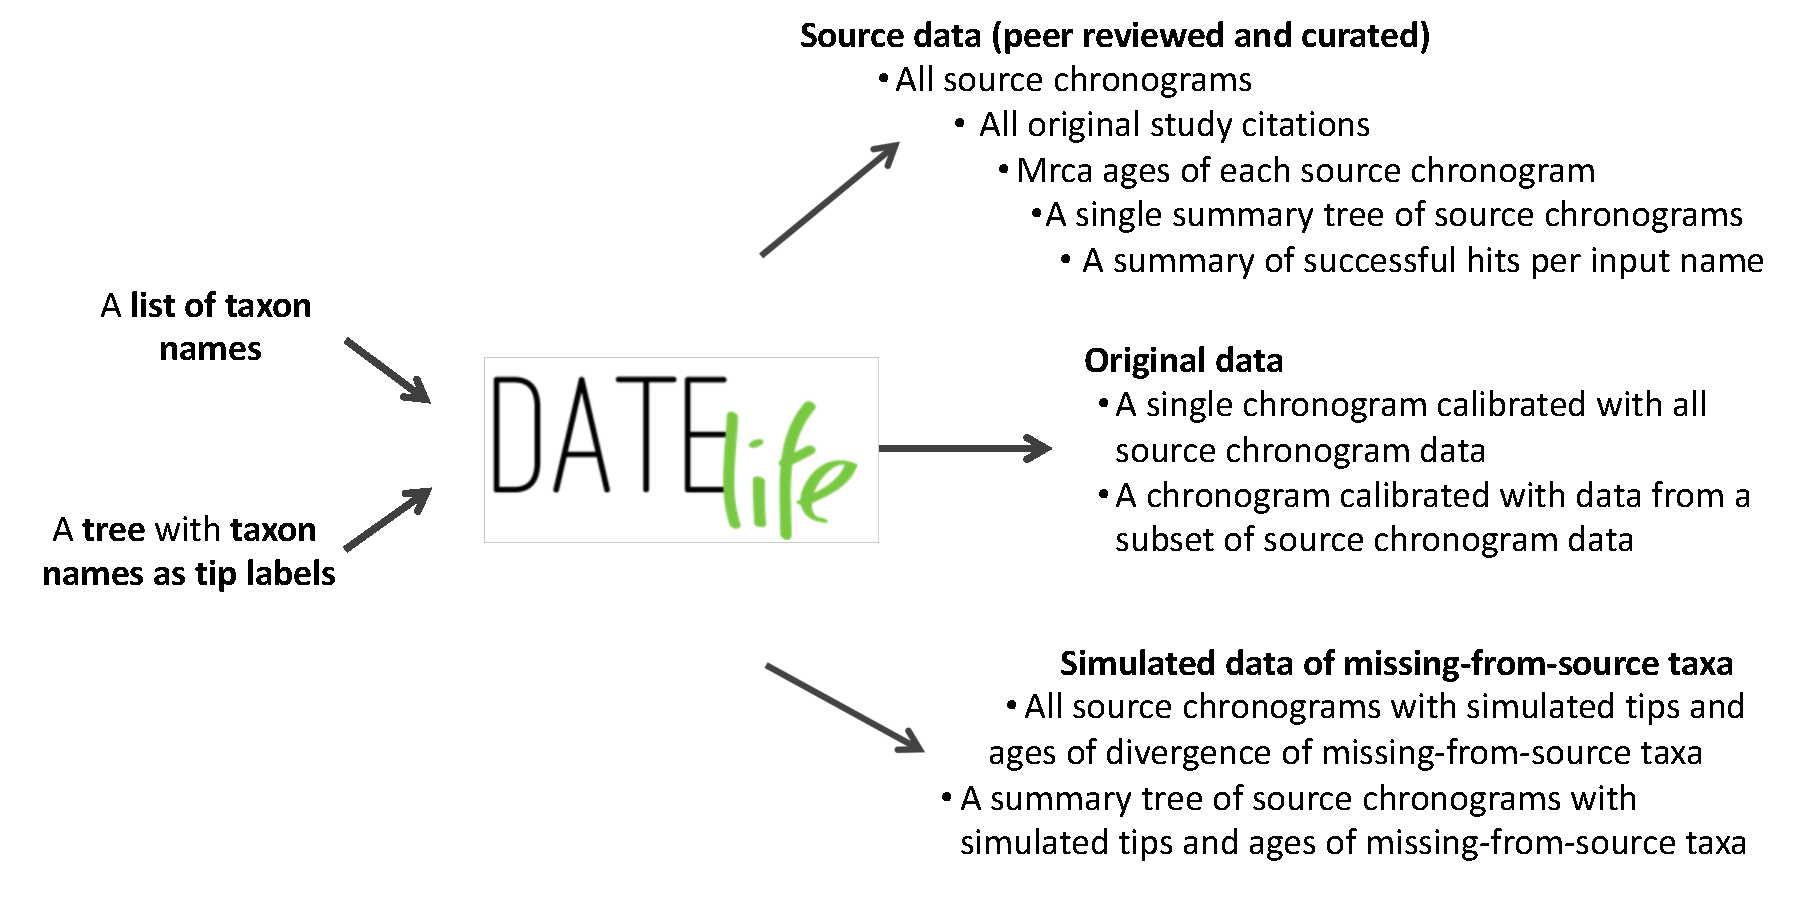
\includegraphics{Fig1.pdf}
\caption{}
\label{fig:workflow}
\end{figure}

\newpage

\begin{figure}[!h]
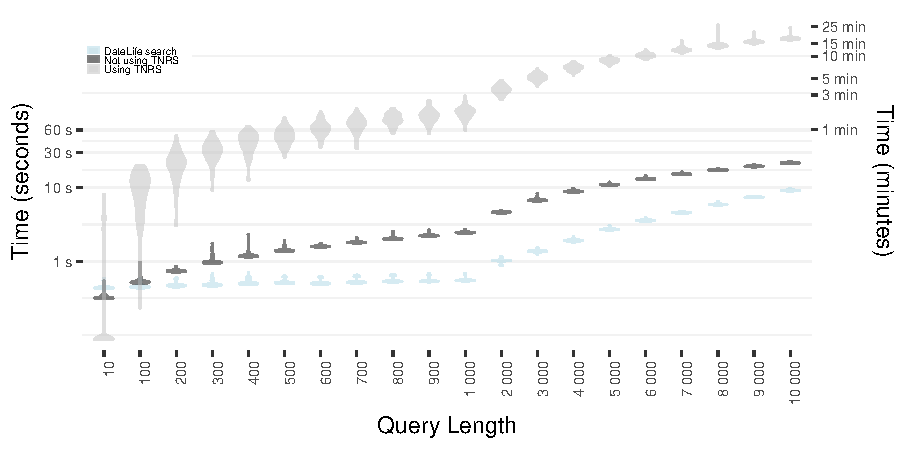
\includegraphics[width=1\linewidth]{fig_runtime1.pdf}
\caption{}
\label{fig:runtime1}
\end{figure}

\newpage

\begin{figure}[!h]
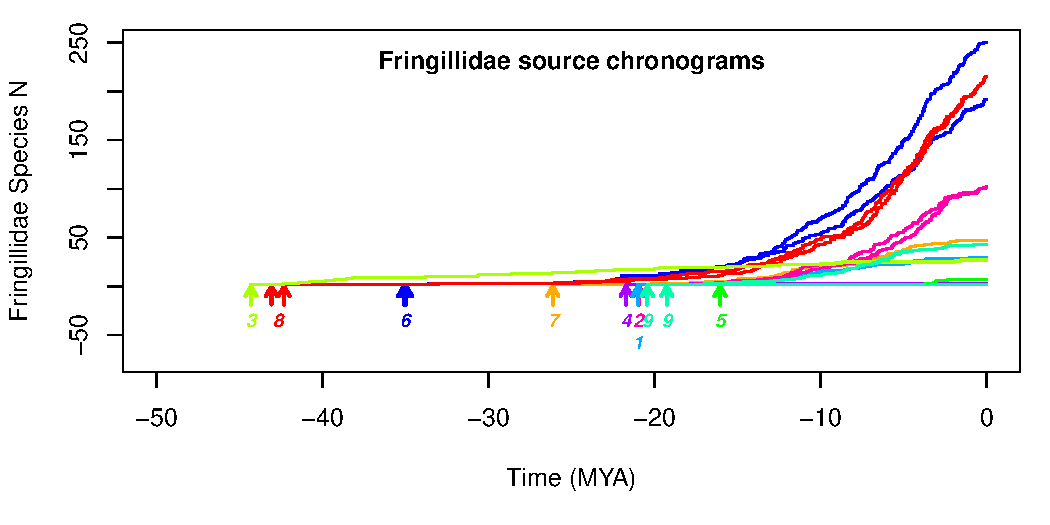
\includegraphics[width=1\linewidth]{fig_schronograms1.pdf}
\caption{}
\label{fig:schronograms1}
\end{figure}

\newpage

\begin{figure}[!h]
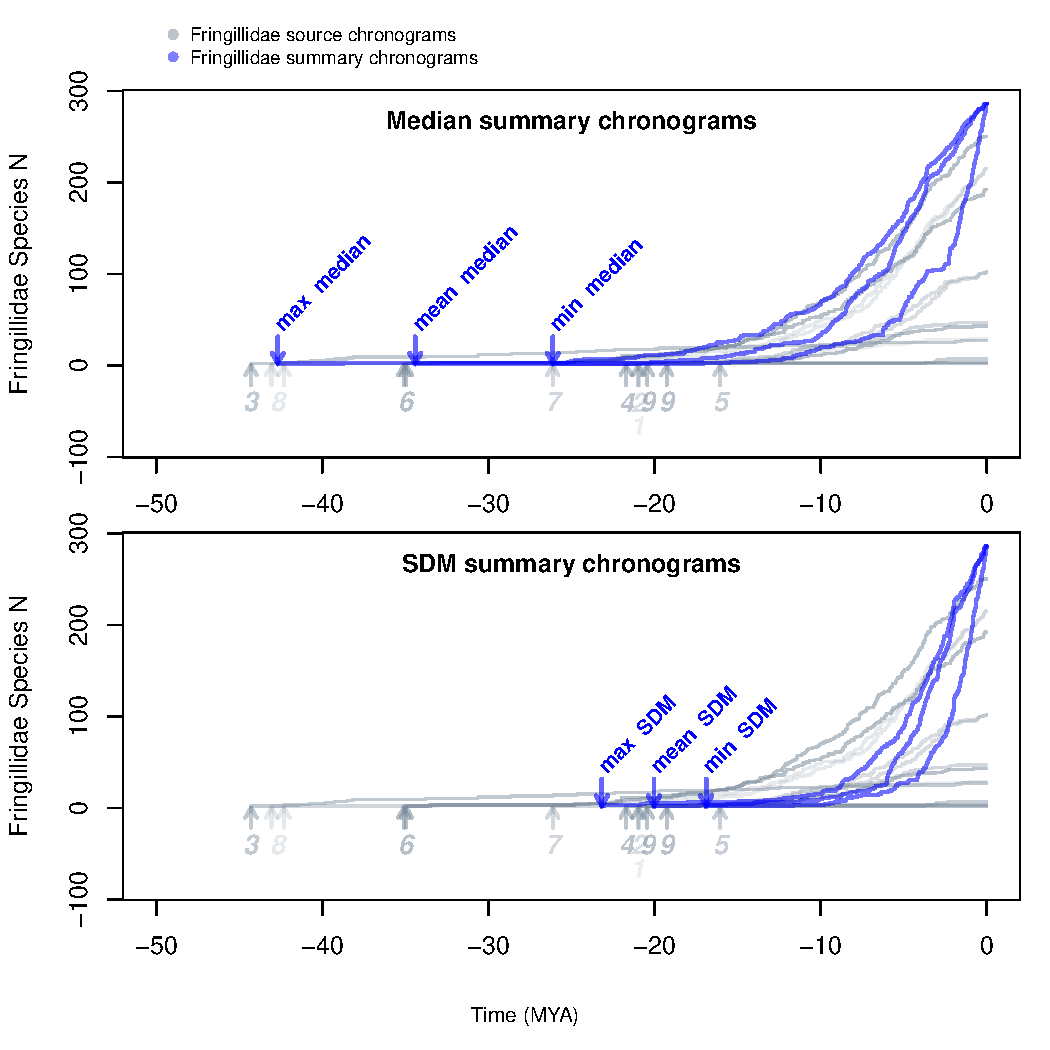
\includegraphics{fig_summaries.pdf}
%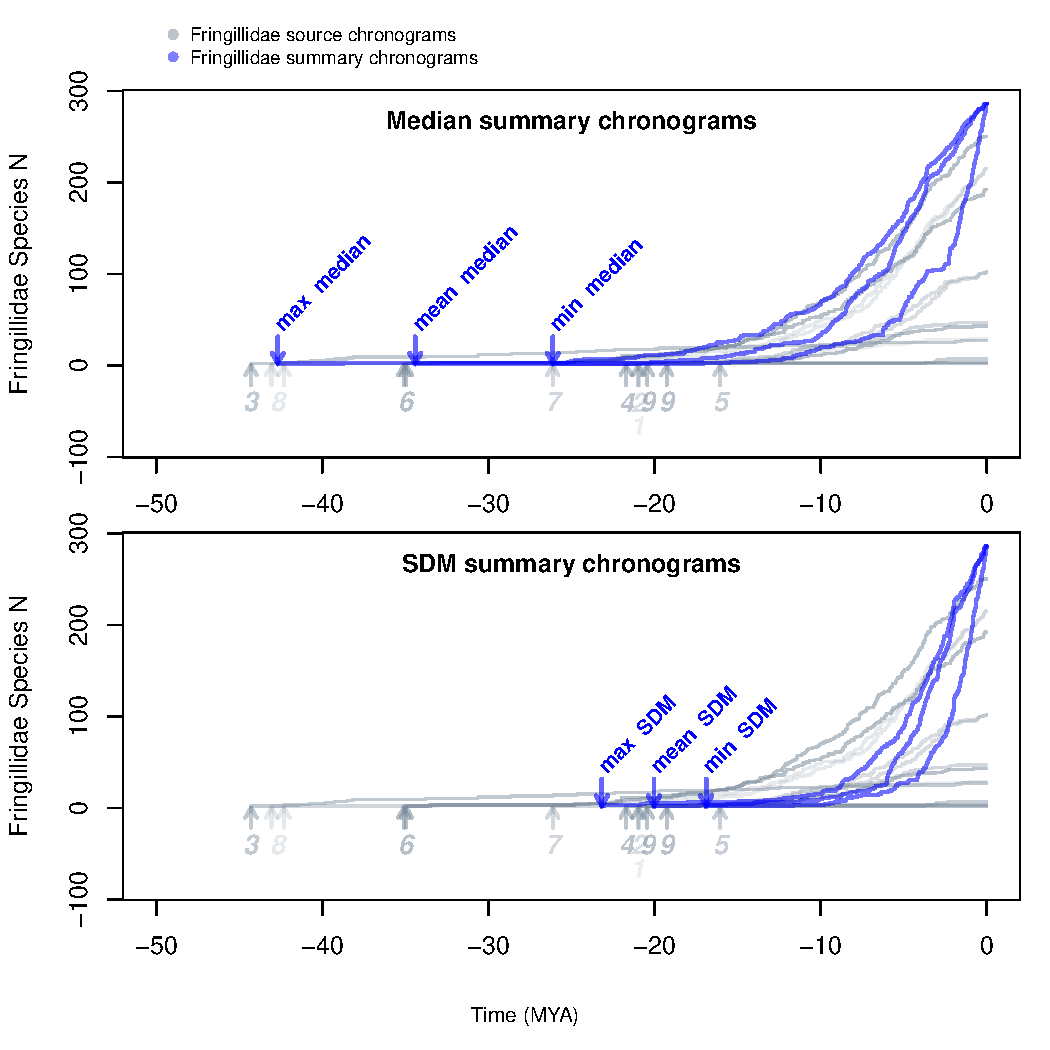
\includegraphics{fig_summaries.pdf}
\caption{}
\label{fig:summaries}
\end{figure}

\newpage

\begin{figure}[!h]
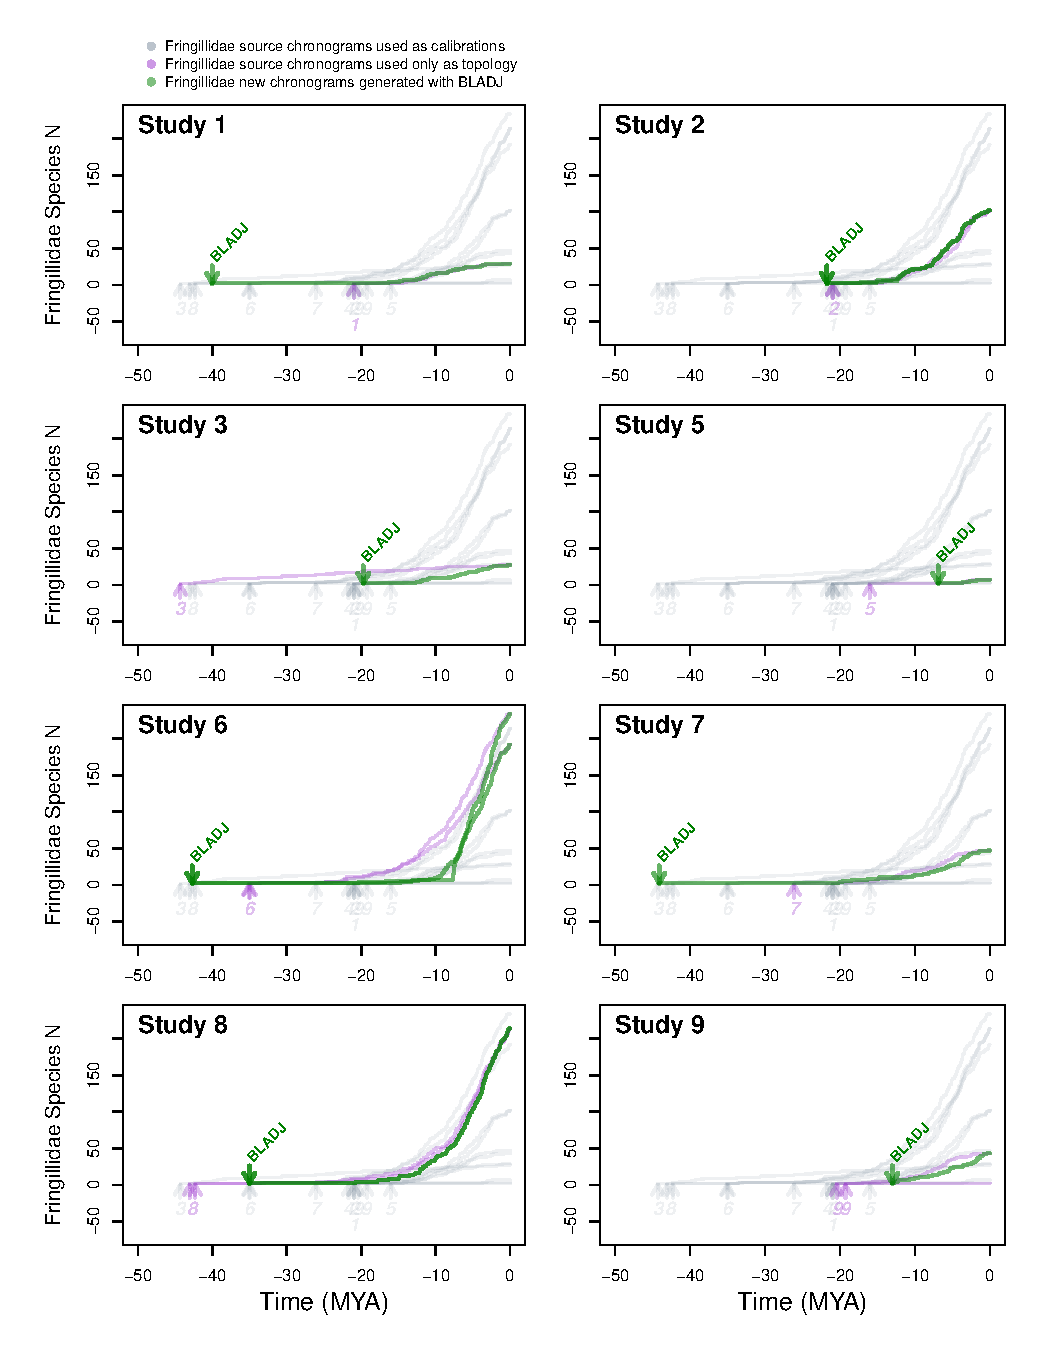
\includegraphics{fig_crossval_bladj.pdf}
\caption{}
\label{fig:cvbladj}
\end{figure}

\newpage

\begin{figure}[!h]
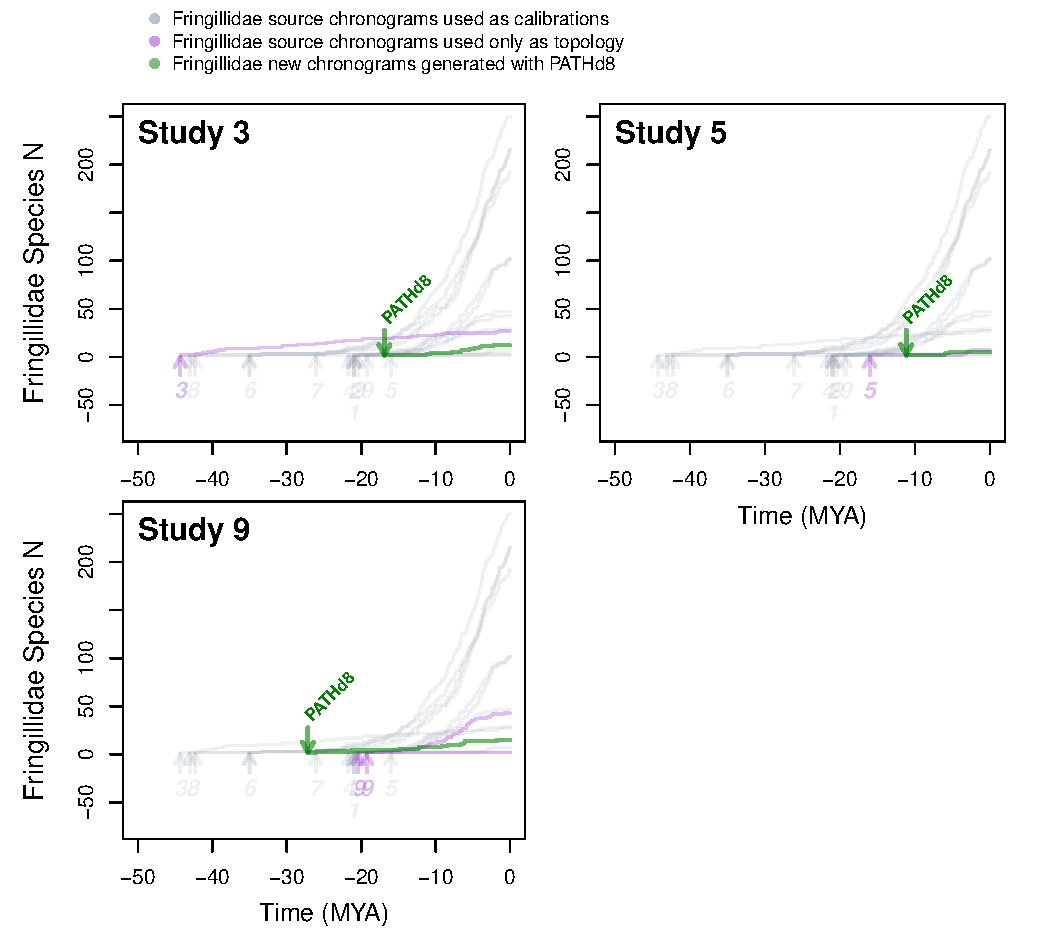
\includegraphics{fig_crossval_boldsumm.pdf}
\caption{}
\label{fig:cvbold}
\end{figure}


\end{document}
